%======================================================================
% L01_uvod_UQWtheta.pdf
%======================================================================
% Poznámky dopsané modrým inkoustem
\providecommand{\modre}[1]{\textcolor{NavyBlue}{#1}}

\section{TD \& SF -- Úvod}
\strana{L01-1}

\begin{itemize}
  \item \textbf{náplň:} popis \kw{makroskopických systémů}
  \begin{itemize}[label={}]
    \item \textbf{SF:} vlastnosti makroskop.\ objektů vyvozuje z mikroskopických vlastností částic (klas.\ nebo kvant.\ hamiltoniánu)
    \item \textbf{TD:} makroskopické vlastnosti popisuje fenomenologicky (nevysvětluje) na základě makroskopických experimentů a pozorování
          \modre{-- bez jakékoliv reference k mikroskopické struktuře!}
  \end{itemize}

  \item \underline{\textbf{TD}} se zabývá rovnováhou, vnitřní energií, \underline{procesy} spojenými s přenosem tepla
        \modre{ovšem bez odkazu na $t$! $\Rightarrow$ spíše TRANSFORMACE}
  \begin{itemize}
    \item[--] přináší pojem \kw{teploty} -- pocit tepla a chladu není subjektivní, mnohé fyzikální vlastnosti látek na \uv{teplotě} závisí (např.\ el.\ odpor, modul pružnosti, \dots)
    \item[--] \uv{opravuje} zákon zach.\ energie v přítomnosti nekonzervativních sil
    \item[--] na rozdíl od SF se nezabývá mikroskopickou strukt.\ objektů, přináší \uline{zcela obecné poznatky platné nezávisle na podstatě látky} -- stejně např.\ pro plyny jako elmg.\ pole nebo i prostoročas(?)
    \item[--] ze stejného důvodu nicméně neumí poskytnout vodítka k mikroskopické interpretaci pozorování
    \item[--] popis konkrétních systémů je možný jen na základě \underline{stavových rovnic} dodaných jinou teorií nebo experimentem
  \end{itemize}

  \item \underline{\textbf{SF}} -- vyvozuje makroskopické vlastnosti z mikroskopického modelu na základě teorie pravděpodobnosti
        \modre{(klas.\ vs.\ kvantová pravděpodobnost: stat.\ soubor vs.\ měření v QM)}
  \begin{itemize}
    \item[--] umožňuje jak popis konkrétních systémů tak vyvození obecných závěrů
          \modre{(ovšem dokázat skutečnou obecnost těchto závěrů může být obtížnější)}
    \item[--] přesto nemůže TD zcela nahradit; minimálně jsou základní východiska SF lépe pochopitelná až v kontextu poznatků TD
  \end{itemize}
\end{itemize}

-- srov.\ kinetická teorie plynů

%----------------------------------------------------------------------
\providecommand{\zelene}[1]{\textcolor{OliveGreen}{#1}}
\subsection{Makroskopická a mikroskopická pozorování}
\strana{L01-2}

\marginpar{\raggedright\scriptsize\modre{mikro/makro charakter není zcela objektivní \uv{vlastnost} systému, proto lépe charakt.\ ve vztahu k pozorovateli (např.\ spojité systémy -- pole -- kde není k dispozici nic jako \#částic)}}
\begin{itemize}
  \item \underline{\textbf{makro}} -- dostupné lidským smyslům (třebaže vylepšeným technologií)
  \begin{itemize}
    \item[--] makroskopické škály lze tedy definovat např.\ na základě viditelného světla (\pozn{$\bar e$} mikroskop již nelze považovat za prodloužení smyslů\dots?)
    \[ \vzorec{d_M \sim 5\cdot 10^{-7}\,\mathrm{m}} \qquad (\lambda = 390\text{--}760\,\mathrm{nm}) \]
    \item[--] časové škály: \quad $\vzorec{\tau_M \sim 10^{-2}\text{--}10^{-3}\,\mathrm{s}}$
  \end{itemize}
  \item \underline{\textbf{mikro}} -- 1 mol plynu za normálních podmínek: $V = 22{,}4\,\ell$
  \begin{itemize}
    \item[--] 1 mol: \quad $N_A \doteq 6{,}02\cdot 10^{23}\,\mathrm{mol}^{-1}$
    \[ \Rightarrow\quad \vzorec{d_\mu \sim 10^{-9}\text{--}10^{-10}\,\mathrm{m}} \qquad (\text{Angström}) \]
    \item[--] čas.\ škály: \quad $\vzorec{\tau_\mu \sim 1\,\mathrm{fs} = 10^{-15}\,\mathrm{s}}$ \\
          (vibrace atomů -- 10--100\,fs, pohyb $\bar e$ -- sub-femto)
  \end{itemize}
\end{itemize}

$\Rightarrow$ v \uv{makroskopickém} objemu odpovídajícímu $d_M$ je přibližně \underline{$10^9$ částic}

$\Rightarrow$ makroskopicky pozorujeme děje, které jsou na mikroskopické škále časově středované $\Rightarrow$ \underline{statické} \\
\quad (srov.\ úplná sada pozorovatelných komutujících s hamiltoniánem v QM)

$\Rightarrow$ \underline{makroskopicky} dostupných/měřitelných \underline{veličin} je jen \underline{velmi málo} ve srovnání s typ.\ $6N_A$ mikro.\ stupňů volnosti
\begin{itemize}
  \item i kdybychom uměli $N_A$ pohybových rovnic vyřešit, výsledek by nám k ničemu nebyl
\end{itemize}

\begin{veta}[Makrostav a mikrostavy]
$\Rightarrow$ makroskopickému stavu systému -- \modre{\kw{makrostavu}} \modre{($\to$ bod ve stav.\ prostoru)} -- tedy zjevně odpovídá mnoho různých \zelene{\textbf{mikrostavů}} \zelene{(bod ve fáz.\ prostoru, $\ket{\psi}\in\mathcal{H}_N$)}, které jsou charakterizovány znalostí $\forall$ mikroskopických stupňů volnosti, ale které na základě makro pozorování neumíme rozlišit
\end{veta}

%----------------------------------------------------------------------
\subsection{Osnova}
\strana{L01-3}

\begin{enumerate}[label=\Roman*)]
  \item \underline{fenomenologická TD} (cf Fermi, Luscombe)
  \begin{enumerate}[label=\arabic*)]
    \item 1.\ TD zákon $\to$ \underline{vnitřní energie}, práce, \underline{teplo}
    \item 0.\ TD zákon (tep.\ rovnováha) $\to$ empirická \underline{teplota}
    \item 2.\ TD zákon (teplo teče jen jedním směrem) $\to$ \underline{entropie} a její vlastnosti
  \end{enumerate}
  \item \underline{axiomatická TD}
  \begin{itemize}
    \item $S = S(U,V,N)$ \quad \dots\ \kw{fundamentální rovnice}
    \begin{itemize}[label=$\to$]
      \item rovnováha
      \item stabilita
      \item fázové přechody
      \item alternativní reprezentace -- TD potenciály
      \item vztahy mezi TD veličinami
      \item vybrané další aplikace
    \end{itemize}
  \end{itemize}
  \item \underline{statistický popis makroskopických systémů}
  \begin{itemize}
    \item mikroskopický hamiltonián \ \& \ $S = k_B\log W$ \quad \modre{(Boltzmann)} \\
          $\Rightarrow$ \quad $S = S(U,V,N)$
          \hfill \modre{přesněji $S = k_B\log\Gamma$, \ $\Gamma$: objem dostupné části fázového prostoru}
  \end{itemize}
\end{enumerate}

%----------------------------------------------------------------------
\subsection{Rovnovážná termodynamika}
\strana{L01-4}

\begin{definice}[Rovnovážná TD]
\underline{rovnovážná TD} -- popisuje stavy makro.\ systému, ve kterých se makroskop.\ měřitelné veličiny nemění a jsou rovny svým (časově) středním hodnotám \\
\hfill -- kvazistatické procesy (viz dále)
\end{definice}

\begin{itemize}
  \item definice \uv{\underline{systému}} vyžaduje jeho oddělení od \uv{\underline{okolí}} \\
        $\Rightarrow$ hranice/\underline{stěny} oddělující systém a okolí, umožňující různé typy interakcí $\Rightarrow$ různé \uv{typy} systémů (izolovaný, otevřený\dots)
  \item nejzásadnější dělení je na stěny
  \begin{itemize}
    \item[] \kw{adiabatické} -- výměna energie je možná pouze mechanickou prací, je-li stěna pohyblivá
            \modre{(jiné typy práce zahrneme později a pojmy upřesníme)}
    \item[] \kw{diatermické} \pozn{diatermální?} -- výměna energie může probíhat i jinak, prostřednictvím makroskopicky nepozorovatelných procesů -- \underline{tepelný kontakt} \\
            (viz např.\ tání ledu v běžné uzavřené nádobě)
  \end{itemize}
  \item pohyblivé stěny umožňují mechanickou interakci
  \item \underline{permeabilní} stěny -- výměna hmoty
\end{itemize}

\begin{center}
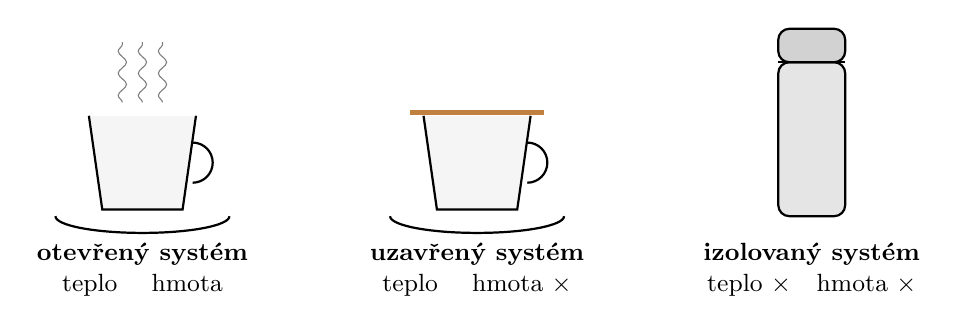
\begin{tikzpicture}[scale=0.85,font=\small]
  % otevřený systém -- hrnek bez víčka, pára
  \begin{scope}[xshift=0cm]
    \draw[thick,fill=gray!8] (-0.8,1.4) -- (-0.6,0) -- (0.6,0) -- (0.8,1.4);
    \draw[thick] (0.75,1.0) arc (90:-90:0.3);
    \draw[thick] (-1.3,-0.1) arc (180:360:1.3 and 0.25);
    \foreach \x in {-0.3,0,0.3}
      \draw[gray,decorate,decoration={snake,amplitude=1.5pt,segment length=8pt}] (\x,1.6) -- (\x,2.5);
    \node[align=center] at (0,-0.9) {\textbf{otevřený systém}\\teplo \checkmark\quad hmota \checkmark};
  \end{scope}
  % uzavřený systém -- hrnek s víčkem
  \begin{scope}[xshift=5cm]
    \draw[thick,fill=gray!8] (-0.8,1.4) -- (-0.6,0) -- (0.6,0) -- (0.8,1.4);
    \draw[thick] (0.75,1.0) arc (90:-90:0.3);
    \draw[thick] (-1.3,-0.1) arc (180:360:1.3 and 0.25);
    \draw[line width=2pt,brown] (-1,1.45) -- (1,1.45);
    \node[align=center] at (0,-0.9) {\textbf{uzavřený systém}\\teplo \checkmark\quad hmota $\times$};
  \end{scope}
  % izolovaný systém -- termoska
  \begin{scope}[xshift=10cm]
    \draw[thick,fill=gray!20,rounded corners=4pt] (-0.5,-0.1) rectangle (0.5,2.2);
    \draw[thick,fill=gray!35,rounded corners=4pt] (-0.5,2.2) rectangle (0.5,2.7);
    \draw[thick] (-0.5,2.2) -- (0.5,2.2);
    \node[align=center] at (0,-0.9) {\textbf{izolovaný systém}\\teplo $\times$\quad hmota $\times$};
  \end{scope}
\end{tikzpicture}
\end{center}
\pozn{v originále vložený obrázek \uv{Thermodynamic Systems} (open / closed / isolated system)}

%----------------------------------------------------------------------
\subsection{Stav termodynamické rovnováhy}
\strana{L01-5}

\begin{definice}[Termodynamická rovnováha]
Makroskopický systém je ve stavu \kw{termodynamické rovnováhy}, pokud se žádné makroskopické veličiny v čase nemění, a tento stav je plně popsatelný malým počtem (TD) parametrů.
\end{definice}

\begin{veta}[Postulát]
\textcolor{Red}{Každý izolovaný makroskopický systém dospěje po dostatečně dlouhém čase do stavu TD rovnováhy, ve kterém se již makroskopicky nemění. Tento stav je určen jen vnějšími parametry (\uv{okraj.\ podmínkami}), jedním vnitřním parametrem a vlastnostmi systému, nikoliv dříve působícími vnějšími vlivy.}
\begin{itemize}[nosep]
  \item[--] \modre{vnější parametry: externě kontrolovatelné (objem, počet částic, vnější mag.\ pole\dots)}
  \item[--] \modre{vnitřní parametr: vnitřní energie nebo teplota (vnější parametry nestačí -- stav systému závisí na tom, kolik je v něm obsaženo energie)}
  \item[--] \modre{vlastnosti systému: vlastnosti popsané stavovými rovnicemi (interagující vs neinteragující částice atp)}
\end{itemize}
\end{veta}

\begin{itemize}[label=$\Rightarrow$]
  \item ve stavu TD rovnováhy si \underline{systém nepamatuje svoji historii}
  \item pro dané hodnoty vnějších a vnitřních par.\ je rovn.\ stav pouze jeden
  \item postulát zde předjímá trochu více, než je nutné, něco \uv{odvodíme}
\end{itemize}
\begin{itemize}
  \item[--] fyzikální systémy obecně paměť mají -- jejich vývoj je odezva na minulou interakci s okolím \\
        $\Rightarrow$ již zde předjímáme, že \underline{vývoj} systému směrem \underline{k rovnováze je nevratný}, v kontrastu se symetrií mikroskopických rovnic
  \item[--] stav TD rovnováhy systém nemůže opustit samovolně, ale pouze v důsledku změny vnějších parametrů/interakcí s okolím
\end{itemize}

\subsection{Popis rovnovážného stavu}
\begin{itemize}
  \item[--] \kw{stavové veličiny} -- makroskopicky měřitelné
  \begin{itemize}
    \item $p, V, N, \vec E, \vec P, \vec H, \vec M, \sigma$ (povrchové napětí), viskozita, el.\ vodivost, \dots
    \item $T, U$ \dots\ intuitivně chápeme, ale striktně vzato budeme teprve definovat
    \item ne všechny jsou nezávislé -- ze znalosti několika málo je možné ostatní odvodit, ať až ze znalosti \underline{stavových rovnic} nebo obecných vztahů, které nám TD poskytne
  \end{itemize}
\end{itemize}

%----------------------------------------------------------------------
\strana{L01-6}
\begin{definice}[Stavové proměnné a stavový prostor]
$\Rightarrow$ nezávislé stav.\ veličiny $\equiv$ \kw{stavové proměnné}, definují \kw{stavový prostor}
\begin{itemize}[nosep]
  \item[--] každý bod stav.\ prostoru odpovídá jednomu možnému rovnovážnému stavu systému
  \item[--] volba nez.\ stav.\ proměnných je do značné míry libovolná a závisí na konkrétním problému, který chceme řešit
  \item[--] ostatní (závislé) veličiny můžeme nazývat \underline{stavovými funkcemi} (jsou to funkce na stav.\ prostoru)
\end{itemize}
\end{definice}

\begin{itemize}
  \item počet nez.\ stav.\ proměnných definuje \underline{dimenzi stav.\ prostoru}
  \begin{itemize}
    \item[--] závisí na charakteru systému (izolovaný, uzavřený, \dots)
    \item[--] \underline{závisí} také \underline{na typu} a přesnosti \underline{dostupných měření}
  \end{itemize}
\end{itemize}

\textbf{Př:} \quad jednokomponentní plyn -- $p, V$ \quad (nebo $T, V$ či $T, p$)

\begin{itemize}
  \item charakter TD veličin:
\end{itemize}
\begin{itemize}[label=$\langle$,leftmargin=2.5em]
  \item \kw{extenzivní} -- jsou úměrné \uv{velikosti} systému (počtu částic/hmotnosti)
  \begin{itemize}[nosep]
    \item[--] aditivní pro nezávislé podsystémy
    \item[--] $N, V, U, M, P, \dots$
  \end{itemize}
  \item \kw{intenzivní} -- nezávislé na množství látky
  \begin{itemize}[nosep]
    \item[--] mají \underline{stejnou hodnotu ve všech částech} systému
    \item[--] $T, p, \vec H, \vec E, \dots$
    \item[--] striktně vzato \underline{definovány pouze v rovnovážném stavu}
  \end{itemize}
\end{itemize}
\begin{itemize}[label=$\langle$,leftmargin=2.5em]
  \item \kw{vnější} -- určeny zobecněnými souřadnicemi částic tvořících okolí systému (lze mezi ně ale řadit také celkový neměnný počet částic, \dots)
  \item \kw{vnitřní} -- určeny zobec.\ souřadnicemi částic systému/jejich hodnoty závisí na vlastnostech daného systému (v jiném systému za stejných podmínek nabývají odlišných hodnot)
\end{itemize}

%----------------------------------------------------------------------
\newpage
\section{První termodynamický zákon}
\strana{L01-7}

\subsection{Adiabatické a jiné stěny}
\begin{itemize}
  \item \underline{stěny} definují, co je \underline{systém} a co je \underline{okolí}
  \begin{enumerate}[label=\arabic*)]
    \item adiabatické
    \item diatermální
    \item propustné (permeabilní)
  \end{enumerate}
  \item obecně je změna stavu systému vyvolána interakcí s okolím: systém je vyveden z rovnováhy a ustaví se nový r.\ stav
  \item charakter stěn definuje možné typy interakcí
\end{itemize}

\subsection{Práce}
\begin{itemize}
  \item obecně \underline{práci definuji} jako interakci s okolím, kterou lze spojit s kontrolovatelnou změnou nějaké měřitelné makroskopické (extenzivní) veličiny \modre{(vnějšího parametru)}, neboli jedná se o interakci, které \uv{rozumím} -- umím ji popsat v rámci nějaké části klas.\ fyziky mimo TD
  \item[--] zároveň ale víme, že systém obecně může interagovat s okolím i jinak -- led v nápoji se rozpustí, když dostatečně dlouho počkáme, přestože byl na počátku s tekutinou v rovnováze
  \item experiment ukazuje, že \underline{existují adiabatické stěny} -- je možné systém uzavřít tak, že se jeho stav mění pouze kontrolovaným způsobem, popsatelným známými teoriemi -- \uv{působením práce} \\
        (s dobrou přesností -- např.\ Dewarovy lahve)
        \modre{\dots\ jedná se o idealizaci, ke které se lze libovolně přiblížit -- to je pro TD charakteristické}
  \item 1840' $\to$; \underline{Joule, Carnot, Thomson} (= Rumford)
\end{itemize}

\begin{veta}[Klíčové experimentální zjištění]
\textcolor{Red}{$\Rightarrow$ práce vykonaná na izolovaný systém během přechodu mezi dvěma rovnovážnými stavy $A$ a $B$ nezávisí na způsobu, jakým byla vykonána, ale pouze na koncových stavech $A, B$}
\end{veta}

%----------------------------------------------------------------------
\strana{L01-8}
$\Rightarrow$ implikuje existenci odpovídající stavové veličiny
\begin{definice}[Vnitřní energie]
\[
  \text{\kw{vnitřní energie}}\qquad \vzorec{\Delta U = U(B) - U(A) \equiv W^{ad}}
\]
\end{definice}

\begin{itemize}
  \item stejně jako (mechanická) potenciální energie je i $U$ def.\ až na aditivní konstantu, tj.\ je vztažena vůči \underline{referenčnímu stavu}: \quad $U(A) - U(0) = W^{ad}_{0A}$
\end{itemize}
$\Rightarrow$ fyzikálně významné jsou jen rozdíly vnitřní energie
\begin{itemize}
  \item \textcolor{Red}{aby byla $U$ dobře definována na celém stav.\ prostoru, je nutné, aby bylo možné mezi libovolnými dvěma body přejít \underline{alespoň v jednom směru} pouze působením práce (adiabaticky)}
  \item \pozor{oběma směry to skutečně možné být nemusí!}
\end{itemize}

\begin{priklad}[Př: plyn v nádobě s pístem]
\begin{itemize}[nosep]
  \item mech.\ práci na plynu v nádobě s pístem můžeme konat buď pístem nebo mícháním vrtulkou (viz cvičení)
  \item[--] přechod $(p_0, V_0)\to(p_1, V_0)$ je adiabaticky možný jen pro $p_1 > p_0$ \\
            (další náznak \underline{existence nevratných procesů})
\end{itemize}
\end{priklad}

\begin{itemize}
  \item existence $U$ jako stavové veličiny implikuje existenci \underline{kalorické -- stavové rovnice}
        \[ \vzorec{U = U(X_1,\dots,X_k)} \qquad \text{\modre{$X_i$ -- vnější parametry}} \]
  \begin{itemize}
    \item[--] pro jednokomp.\ tekutinu např.\ $U = U(p,V)$
  \end{itemize}
  \item $U$ je zjevně \underline{extenzivní veličina}
\end{itemize}

\underline{Pozn:} -- dnes umíme existenci vnitřní energie podložit mikroskopickými úvahami; induktivní vyvození výše má ovšem hodnotu ve své obecnosti

%----------------------------------------------------------------------
\subsection{Teplo}
\strana{L01-9}
\begin{itemize}
  \item sejmeme-li adiabatickou izolaci, stav systému a tedy i $U$ se může měnit i jinak než působením práce $\Rightarrow$ def.\ \kw{teplo}
\end{itemize}
\begin{veta}[Zákon zachování energie -- 1.\ TDZ]
\[
  \vzorec{Q \equiv \Delta U - W = W^{ad} - W}
\]
\end{veta}
\begin{itemize}
  \item $Q$ zahrnuje $\forall$ typy interakcí/přenosy energie, které nejsou přímo kontrolovatelné pozorovatelem a spojeny změnou makroskop.\ \modre{(vnějších)} extenzivních veličin
\end{itemize}
\modre{\underline{Pozn:} Takto formulovaná definice naznačuje, že koncept tepla a dělení přenosu energie na $W$ a $Q$ nemusí být zcela objektivně definován a souvisí s \uv{rozlišovací schopností pozorovatele}. Tento pohled bych nicméně nepřeceňoval, lépe je spojovat pojem teplo s \uv{makroskopicky principiálně nepoznatelným}. Přesto -- pojmy makro/mikro jsme spojili spíše s charakterem pozorování/pozorovatele než s vlastnostmi samotného objektu\dots}

\begin{itemize}
  \item znaménková \underline{konvence}: \quad $Q, W > 0$ \dots\ energie teče \underline{do} systému $\Rightarrow \Delta U > 0$
\end{itemize}

$\Rightarrow$ \kw{adiabatický proces} -- proces, při kterém se nevyměňuje teplo
\begin{itemize}
  \item[\pozor{!}] (zatím) nemluvíme o adiabatě jako nadploše ve stav.\ prostoru; srov.\ (izoterma), izochora, izobara -- jsou def.\ konstantností stavové veličiny
  \item \pozor{$Q$ je veličina \underline{dějová}} -- neex.\ funkce $Q = Q(X_1,\dots,X_k)$
\end{itemize}

\subsection{Kvazistatické procesy}
\begin{itemize}
  \item $\Delta U_{AB} = Q + W$ odkazuje pouze na počáteční (A) a koncový (B) stav děje, na průběh neklade žádná omezení
  \item v průběhu děje systém obecně není v rovnováze \\
        $\Rightarrow$ děj nelze charakterizovat trajektorií ve stavovém prostoru
\end{itemize}

%----------------------------------------------------------------------
\providecommand{\dbar}{{\mathchar'26\mkern-12mu d}}
\strana{L01-10}
\begin{definice}[Kvazistatický proces]
\kw{kvazistatický proces} -- idealizace velmi pomalého$^{\circledast}$ děje, během kterého systém prochází sérií infinitezimálně blízkých rovnovážných stavů; syst.\ je v každém okamžiku v rovnováze $\Rightarrow$ lze popsat trajektorií ve stav.\ prostoru

{\small $^{\circledast}$ pomalý vzhledem k typ.\ relax.\ časům, může být i dosti rychlý (někdy např.\ stačí pomalejší než zvuk)}
\end{definice}

\underline{Pozn:} v rovn.\ TD čas nevystupuje jako proměnná, kvazist.\ procesy jsou \uv{nekonečně pomalé} (výjimka: Ingo Müller) \\
\modre{$\bullet$ lze také mluvit o transformacích}

\begin{itemize}
  \item 1.\ TDZ v dif.\ tvaru pro kvazistat.\ proces ($\lim B\to A$)
  \[ \vzorec{\dd U = \dbar Q + \dbar W} \]
  \item $\dd$ vs.\ $\dbar$:
  \begin{itemize}
    \item $\dd U = \displaystyle\sum_{i=1}^{k}\Big(\pdv{U}{X_i}\Big)\dd X_i$ \quad \underline{je úplný diferenciál} funkce $U = U(X_1,\dots,X_k)$ na stav.\ prostoru
    \item $\dbar Q = \sum_i A_i(X_1,\dots,X_k)\,\dd X_i$ \quad \underline{není úplný diferenciál} $\Rightarrow$ $\nexists\, Q = Q(X_1,\dots,X_k)$
    \[
      \pdv{A_i}{X_j} \neq \pdv{A_j}{X_i} \quad\Leftrightarrow\quad \oint\dbar Q \neq 0
    \]
  \end{itemize}
  \item $\dbar\omega = \sum_i A_i(X_1,\dots,X_k)\,\dd X_i$ je obecně lineární diferenciální (\kw{Pfaffova}) forma
  \begin{itemize}
    \item podmínky integrability, integrační faktor -- viz cvičení
          \hfill \modre{$\operatorname{rot}(\mu\vec A) = 0$; \ \uv{integrabilní verze tepla}: entropie}
  \end{itemize}
  \item \underline{diferenciál stavové veličiny} je \underline{vždy úplný}
  \begin{itemize}
    \item[--] odráží \underline{absenci paměti} systému, kterou jsme postulovali -- rovn.\ stav nezávisí na cestě, po které do něj systém dospěl
  \end{itemize}
\end{itemize}

%----------------------------------------------------------------------
\strana{L01-11}
\begin{veta}[$\Rightarrow$ První termodynamický zákon]
\[ \vzorec{\dd U = \dbar Q + \dbar W} \]
\begin{itemize}[nosep]
  \item \modre{existuje vnitřní energie jako stavová veličina (vlastnost rovnovážného systému)}
  \item \modre{teplo a práce jsou formy přenosu energie, nikoliv energie jako takové (je možné měnit teplo na práci a naopak)}
        \quad \textcolor{Red}{$\bullet$ nahrazuje kalorickou teorii (teplo jako zachovávající se fluidum)}
\end{itemize}
\end{veta}

\underline{Pozn:}
\begin{itemize}
  \item formulace 1.\ zákona resp.\ existence $U$ závisí na možnosti uzavřít systém adiabatickými stěnami $\Rightarrow$ v tuto chvíli se omezujeme na \underline{uzavřené systémy} (změnu $U$ spoj.\ s výměnou látky nelze přímočaře rozdělit a $Q$ a $W$; otevřený systém nelze adiabaticky izolovat)
  \item $U$ je dobře def.\ za předpokladu, že mezi lib.\ dvěma stavy lze přejít adiabaticky alesp.\ v 1 směru \\
        $\to$ na úrovni TD to nelze nijak dokázat, existence $U$ je tedy jedním ze sdělení prvního zákona a je třeba ji chápat jako postulát
  \item dělení na \underline{práci} a \uwave{teplo} odpovídá dělení na \underline{makro}- a \uwave{mikroskopickou} pozorovatelnost \\
        (viz také \modre{modrá poznámka výše})
\end{itemize}

%----------------------------------------------------------------------
\subsection{Práce v kvazistatickém procesu}
\strana{L01-12}
\begin{itemize}
  \item obecně je práce spojena se změnou extenzivní makroskopické veličiny
\end{itemize}

\begin{minipage}[t]{0.45\textwidth}
\[
  \Rightarrow\quad \vzorec{\dbar W = \sum_j y_j\,\dd X_j} \quad \modre{(+)}
\]
\fcolorbox{NavyBlue}{white}{\begin{minipage}{0.9\linewidth}\small\modre{
$\bullet$ možná by bylo intuitivnější definovat $X_j$ jako \uv{vnější} spíše než \uv{extenzivní} parametry, nicméně:
\begin{enumerate}[nosep,label=\arabic*)]
  \item až na výjimky je to totéž
  \item naše volba je lépe matematicky uchopitelná
  \item nakonec to bude tak trochu jedno
\end{enumerate}}\end{minipage}}
\end{minipage}
\hfill
\begin{minipage}[t]{0.5\textwidth}
\begin{itemize}
  \item $X_j$ \dots\ \kw{zobecněné posunutí} -- extenzivní TD veličiny
  \item $y_j$ \dots\ \kw{sdružená zobecněná síla} (intenzivní vel.)
\end{itemize}
\[ [\,y_jX_j\,] = \text{energie} \]
\end{minipage}

\begin{itemize}
  \item \underline{explicitní výrazy pro práci}

  \begin{tabular}{@{\quad$\bullet$ }ll}
    změna objemu tekutiny & $\dbar W = -p\,\dd V$ \\
    změna plochy povrchu (blána) & $\dbar W = \sigma\,\dd\Sigma$ \\
    deformace tělesa & $\dbar W = \sigma_{ij}\,\dd\varepsilon_{ij}$ \\
    polarizace dielektrika & $\dbar W = \vec E\cdot\dd\vec P$ \\
    magnetizace & $\dbar W = \vec H\cdot\dd\vec M$ \quad (Callen, Luscombe)
  \end{tabular}
\end{itemize}

\underline{Pozn:}
\begin{itemize}
  \item spojení $\dbar W = \sum y_i\,\dd X_i$ se změnami \underline{extenzivních} veličin je do značné míry paradigma, které (zdánlivě) upřednostňuje ext.\ veličiny před intenzivními -- a priori je vybírá jako přirozeně nezávislé
  \item výhody ext.\ veličin:
  \begin{itemize}[label=$\to$]
    \item nesou informaci o velikosti systému
    \item (obvykle) jsou definovány i mimo rovnováhu, na rozdíl např.\ od tlaku
  \end{itemize}
  \item viz také \modre{3)} výše
  \item elmg.\ systémy charakteristické tím, že $\vec M$ ($\vec P$) neumíme kontrolovat přímo (neex.\ příslušné \uv{restriktivní stěny}), ale kontrolujeme je skrze vnější pole $\vec H$ ($\vec E$)
\end{itemize}

%----------------------------------------------------------------------
\newpage
\section{Nultý termodynamický zákon a empirická teplota}
\strana{L01-13}

\begin{definice}[Vzájemná TD rovnováha]
\kw{Vzájemná TD rovnováha} -- dva systémy, které se nacházejí v rovnovážných stavech, jsou ve vzájemné rovnováze$^{\circledast}$, pokud po uvedení do vzájemného kontaktu nedojde k žádné změně makroskopických TD veličin

{\small\modre{$^{\circledast}$ charakter rovnováhy závisí na charakteru kontaktu/typu interakce, neboli na charakteru stěn; v TD má speciální význam tepelná výměna (diaterm.\ stěny) $\Rightarrow$ tepelná rovnováha}}
\end{definice}

\begin{veta}[Nultý termodynamický princip]
vztah \underline{tepelné} rovnováhy je tranzitivní. \hfill {\small (ie, jedná se o relaci ekvivalence -- zjevně $A\sim A$)}
\[
  \fcolorbox{Red}{white}{\parbox{0.8\linewidth}{Je-li systém $A$ v rovnováze s $B$ a zároveň s $C$, potom i $B$ je v rovnováze s $C$.}}
\]
\end{veta}
\textcolor{OliveGreen}{\small Maxwell: \uv{Teplo je jediného druhu}: jsou-li syst.\ odděl.\ diaterm.\ stěnou v rovnováze, budou v rovnováze i po oddělení jinou diaterm.\ stěnou. Srov., že totéž nemusí platit pro polopropustné stěny propouštějící různé částice.}

\subsection{Empirická teplota}
\begin{itemize}
  \item[--] \underline{princip teploměru} je založen na nultém principu: teploměr ($A$) uvedu do \textsuperscript{tepelné} rovnováhy s $B$ \pozn{ie, diaterm.\ stěna}; následně je $A$ uvedeno do kontaktu s $C$ a pokud nedojde k žádné makroskopické změně, potom je $B$ v rovnováze s $C$ \\
            (předpokládám $A \ll B, C$ $\Rightarrow$ stav $B$ se v prvním kroku nezmění)
  \item \underline{stavová rovnice} (termická)
  \begin{itemize}
    \item[--] uvažujme jednokomponentní plyny, jejichž stav je charakterizovaný dvojicí $p, V$
    \item[--] jestliže $A, B$ jsou v tepelné rovnováze, potom $p_A, V_A, p_B, V_B$ nemohou být $\forall$ nezávislé $\Rightarrow$ $\exists$ vztah \\
          \modre{\small (každý mód interakce snižuje počet st.\ volnosti o 1; zde k interakci nikde nedochází, ale kdyby mohlo, nic by se nestalo $\Rightarrow$ stavy jsou svázány)}
          \[
            A\sim B \ \Rightarrow\ F_{AB}(p_A,V_A,p_B,V_B) = 0 \quad\Leftrightarrow\quad p_A = f_{AB}(V_A,p_B,V_B)
          \]
    \item[--] analogicky
          \[
            A\sim C \ \Leftrightarrow\ F_{AC}(p_A,V_A,p_C,V_C) = 0 \quad\Leftrightarrow\quad p_A = f_{AC}(V_A,p_C,V_C)
          \]
    \item[--] \underline{tranzitivnost} $\Rightarrow$ \quad $B\sim C \ \Leftrightarrow\ \exists\, F_{BC}(p_B,V_B,p_C,V_C) = 0$
  \end{itemize}
\end{itemize}

%----------------------------------------------------------------------
\strana{L01-14}
\begin{itemize}
  \item dostáváme tedy \quad \modre{\small ($p_C = \dots$ vyjádřeno z obou stran)}
  \[
    f_{AB}(V_A,p_B,V_B) = f_{AC}(V_A,p_C,V_C) \quad\Leftrightarrow\quad F_{BC}(p_B,V_B,p_C,V_C) = 0
  \]
  \item $F_{BC}$ nezávisí na $V_A$ $\Rightarrow$ závislost na $V_A$ na levé straně musí vypadnout $\Rightarrow$
  \[
    \left.\begin{aligned}
      f_{AB} &= \phi_B(p_B,V_B)\,\alpha(V_A) + \beta(V_A) \\
      f_{AC} &= \phi_C(p_C,V_C)\,\alpha(V_A) + \beta(V_A)
    \end{aligned}\right\}
    \quad\Rightarrow\quad \phi_B(p_B,V_B) = \phi_C(p_C,V_C)
  \]
  \item prohozením rolí $A\leftrightarrow B$ dostáváme i
  \[
    \fcolorbox{Red}{white}{$\displaystyle \phi_A(p_A,V_A) = \phi_B(p_B,V_B) = \phi_C(p_C,V_C) = \vartheta$}
    \qquad\text{\small\dots\ \uv{nová} stavová funkce $\to$ veličina}
  \]
  \item $\vartheta = \phi_i(p_i,V_i)$ je \underline{termická stavová rovnice} pro syst.\ \uv{$i$}
        \quad \modre{$\{p_A,V_A\}$ a $\{p_B,V_B\}$ a $\{p_C,V_C\}$ mohou být jiné typy veličin!} \\
        $\Rightarrow$ $\vartheta$ \dots\ \kw{empirická teplota}
  \item teplota je \underline{charakteristika rovnovážného stavu}, není to vlastnost mikroskopických částic látky (srov.\ kin.\ teorie plynů a $T\leftrightarrow\langle E_k\rangle$ \dots\ TD definice je mnohem obecnější)
        \modre{zde $\vartheta$/$T$ je svázána s kolektivní char.\ celého souboru částic}
  \item vzájemná rovnováha je charakterizována stejnou teplotou $\vartheta$
  \item $\vartheta$ je \underline{empirická} -- je určena vlastnostmi konkrétní látky, kterou použijeme jako teploměr, a konkrétní charakteristikou, kterou měříme (výška sloupce = objem)
  \item postup lze zopakovat; pro obecné systémy charakt.\ pomocí $k$ proměnných $X_1,\dots,X_k$ \\
        \hspace*{4cm} $\Rightarrow$ dostaneme opět \quad $\vzorec{\vartheta = \phi_i(X_1,\dots,X_k)}$
  \item \modre{\underline{izoterma}:} \ $\vartheta(X_1,\dots,X_k) = \vartheta_0$ \quad \dots\ nadplocha ve stav.\ prostoru
  \item teplota je \underline{intenzivní veličina} -- systém můžeme myšleně rozdělit na podsystémy, které jsou samozřejmě v rovn.\ $\Rightarrow$ $\vartheta$ stejná ve $\forall$ bodech systému
\end{itemize}

%----------------------------------------------------------------------
\strana{L01-15}
\begin{priklad}[Př: teploměr, plyn a Isingův magnet {\normalfont\small (celá stránka modře)}]
\modre{
\begin{tabular}{lll}
$A$: & teploměr & $p_A, V_A$ \\
$B$: & plyn & $p_B, V_B$ \\
$C$: & Ising & $M_C, H_C$
\end{tabular}
\begin{align*}
  B\sim A \ &\Rightarrow\ \exists\,F_{AB}(p_A,V_A,p_B,V_B) = 0
     \ \Rightarrow\ V_A = f_{AB}(p_A,p_B,V_B) \\
  C\sim A \ &\Rightarrow\ \exists\,F_{AC}(p_A,V_A,M_C,H_C) = 0
     \ \Rightarrow\ V_A = f_{AC}(p_A,M_C,H_C) \\
  &\Downarrow\ \text{0.\ TDZ} \\
  C\sim B \ &\Rightarrow\ \exists\,F_{BC}(p_B,V_B,M_C,H_C) = 0 \\
  &\Updownarrow\ \text{equiv.\ rovnost} \\
  f_{AB}(p_A,p_B,V_B) &= f_{AC}(p_A,M_C,H_C) \\
  &\Downarrow\ \text{závislost na $p_A$ musí vypadnout} \\
  \Rightarrow\quad f_{AB} &= \phi_B(p_B,V_B)\,\alpha(p_A) + \beta(p_A) \\
  f_{AC} &= \phi_C(M_C,H_C)\,\alpha(p_A) + \beta(p_A)
\end{align*}
\[
  \Rightarrow\quad \fbox{$f_{AB} = f_{AC} \ \Leftrightarrow\ \phi_B(p_B,V_B) = \phi_C(M_C,H_C)$}
\]}
\textcolor{Red}{$\Rightarrow$ \quad $\vartheta = \phi_B(p_B,V_B) = \phi_C(M_C,H_C)$ je \underline{empirická teplota} a $\phi_i$ \underline{termická stav.\ rovnice}}
\end{priklad}

%----------------------------------------------------------------------
\strana{L01-16}
\begin{itemize}
  \item[--] Joule: pro id.\ plyn \ $U = U(\vartheta)$ \dots\ exp.\ fakt \quad \modre{\small ($\vartheta$ \dots\ empirická teplota)}
  \item[--] \modre{kalorická a termická $[\vartheta = \vartheta(X_1,\dots,X_k)]$ stavové rovnice nejsou zcela nezávislé -- funkční tvar jedné klade omezení na druhou, jak uvidíme po zavedení entropie} \modre{\small($\curvearrowright$ viz id.\ plyn níže)}
\end{itemize}

\begin{veta}[$\Rightarrow$ Nultý zákon]
Nultý zákon implikuje existenci teploty jako charakt.\ rovnovážného stavu a také stavové rovnice -- funkčního vztahu mezi stavovými parametry.
\end{veta}

\subsection{Stavové rovnice konkrétních systémů}
\begin{enumerate}[label=\arabic*)]
  \item \underline{ideální plyn}
  \begin{itemize}
    \item idealizovaný model neint.\ částic, stav char.\ 2 proměnnými
    \[
      \vzorec{\vartheta = \frac{pV}{Nk_B}}\ \ (= T) \qquad k_B = 1{,}38\cdot 10^{-23}\,\mathrm{J/K}
      \quad \text{\small (ještě \uv{nevíme}, co je K\dots)}
    \]
  \end{itemize}

  \item \underline{van der Waalsův plyn}
  \[
    \vzorec{p = \frac{Nk_BT}{(V - Nb)} - a\Big(\frac{N}{V}\Big)^2}
    \qquad
    \begin{aligned}
      b &> 0 \text{ -- korekce na kon.\ objem částic} \\
      a &> 0 \text{ -- efekt přitažlivé interakce mezi částicemi}
    \end{aligned}
  \]
  \begin{itemize}
    \item[-] pokles tlaku vlivem interakce je úměrný pstí interakce dvou částic $\propto$ kvadrát hustoty
  \end{itemize}

  \item \underline{viriálový rozvoj} -- obecnější popis odchylek od id.\ plynu
  \[
    p = \frac{Nk_BT}{V}\Big[1 + \Big(\frac{N}{V}\Big)B_2(T) + \Big(\frac{N}{V}\Big)^2B_3(T) + \dots\Big]
  \]
  (vdW: \ $B_2(T) = b - \frac{a}{kT}$, \ $B_{i>2}(T) = b^{i-1}$)

  \item \underline{ideální paramagnet}
  \[
    M = Nm\,\mathcal{L}\Big(\frac{\mu_0 mH}{k_BT}\Big)
    \qquad
    \begin{aligned}
      m &\dots \text{mg.\ moment částice} \\
      H &\dots \text{int.\ mg.\ pole} \\
      \mathcal{L}(x) &= \coth x - \tfrac1x \quad \text{\kw{Langevinova funkce}}
    \end{aligned}
  \]
  \pozn{v originále zapsáno cotg\,$x$}
  \begin{itemize}
    \item[-] $T\nearrow$ \ $\Rightarrow$ \ $\mathcal{L}(x)\sim\frac{x}{3}$ \ $\Rightarrow$ \ $\vzorec{M = \frac{C}{T}H}$ \quad \kw{Curieho zákon}
  \end{itemize}
\end{enumerate}

%----------------------------------------------------------------------
\strana{L01-17}
\underline{Pozn:}
\begin{enumerate}[label=\arabic*)]
  \item nultý zákon (tranzitivnost tepelné rovnováhy) v sobě implicitně obsahuje omezení platnosti budované teorie:
  \begin{itemize}[label=$\to$]
    \item předpokládá, že oddělením/spojením dvou systémů v rovnováze nedojde ke změně jejich rovnovážného TD stavu $\Leftrightarrow$ interakční energie musí být zanedbatelná
  \end{itemize}
  $\Rightarrow$ energie systému musí být aditivní přes podsystémy,
  \[ \vzorec{U = \sum_\alpha U_\alpha} \]
  \begin{itemize}
    \item mikroskopicky toto vyžaduje krátko-dosahovou interakci, aby se výměny energie mezi podsystémy \uv{účastnily} jen objemově zanedbatelné vrstvy v místě kontaktu
  \end{itemize}
  $\Rightarrow$ \pozor{např.\ gravitace je problém\dots}
  \hfill \textcolor{Red}{\uv{4.\ TDZ: $\forall$ TD parametry jsou buď extenzivní nebo intenzivní} $\Rightarrow$ omezení na krátkodosah.\ interakci}

  \item uvedený 1.\ postulát se někdy upřesňuje na postuláty dva:
  \begin{enumerate}[label=\Roman*)]
    \item Každý izolovaný systém po jisté době přejde do rovn.\ stavu a již z něj samovolně nevyjde.
    \item Homog.\ systém v rovnováze je charakterizovatelný hodnotami vnějších parametrů \& jediným vnitřním $(U,\vartheta,\dots)$
  \end{enumerate}
  \begin{itemize}
    \item II je někdy interpretováno jako důsledek I a 0.\ TDZ, neboli je v tom zmatek; navíc to takto formulováno zase tolik prakticky stejně nepomáhá
    \item uvidíme, že definice práce přes $\dbar W = \sum y_i\,\dd X_i$
          \[ \dd U = \dbar Q + \dbar W \]
          povede k poznání, že rovn.\ stav je charakterizován vnitřní energií $U$ a ext.\ veličinami $X_i$, které jsou spojeny s jednotlivými dostupnými módy výměny energie
    \item teplo je potom přenos energie indukovaný rozdílem teplot, který zprostředkovává přechod do vzájemné tepelné rovnováhy, stejně jako mech.\ práce je indukována rozdílem sil/tlaků
  \end{itemize}
\end{enumerate}

